\documentclass[11pt, twocolumn]{article}

\usepackage[spanish]{babel}
\usepackage[none]{hyphenat}
\usepackage[left=1.5cm, right=1.5cm, top = 2cm, bottom=2.5cm]{geometry}
\usepackage{enumitem}
\usepackage{longtable}
\usepackage{multirow, makecell}
\usepackage{listings}
\usepackage{color}
\usepackage{graphicx}
\usepackage{subcaption}
\usepackage{parskip}
\usepackage[hidelinks]{hyperref}
\usepackage{fancyhdr}
\usepackage[export]{adjustbox}

\newcommand{\linejump}{\hfill \break}
\renewcommand{\thefootnote}{\fnsymbol{footnote}}

\definecolor{dkgreen}{rgb}{0,0.6,0}
\definecolor{gray}{rgb}{0.5,0.5,0.5}
\definecolor{mauve}{rgb}{0.58,0,0.82}
\lstset{
  language=Java,
  aboveskip=3mm,
  belowskip=3mm,
  showstringspaces=false,
  columns=flexible,
  basicstyle={\tiny\ttfamily},
  numbers=none,
  numberstyle=\tiny\color{gray},
  keywordstyle=\color{blue},
  commentstyle=\color{dkgreen},
  stringstyle=\color{mauve},
  breaklines=true,
  breakatwhitespace=true,
  tabsize=3
}

\sloppy
\setlength{\parindent}{0cm}
\setlength{\columnsep}{0.5cm}
\decimalpoint
\graphicspath{{img/}}

\hypersetup{colorlinks=true, urlcolor=blue, citecolor=blue}
\urlstyle{same}

\pagestyle{fancyplain}
\fancyhf{}
\fancyhead[L]{\scriptsize 
  Universidad Nacional Autónoma de México \\
  Laboratorio de Programación Orientada a Objetos \\
  M.C. Leonardo Ledesma Dominguez
}
\fancyhead[R]{\thepage}


\begin{document}
  \twocolumn[
    \centering
    Acosta Porcayo Alan Omar, Gutiérrez Grimaldo Alejandro, Medina Villa Samuel

    \linejump

    \LARGE \textbf{Práctica 2. Fundamentos y sintaxis del lenguaje} \\
    
    \linejump
  ]
      
  \footnotetext{
    \scriptsize 
    Acosta Porcayo Alan Omar Ing. en Computación 320206102 \\
    Gutiérrez Grimaldo Alejandro Ing. en Computación 320282098 \\
    Medina Villa Samuel Ing. en Computación 320249538
  }
        
  \fancyfoot{}

  \section*{Resumen}
  El propósito de esta práctica es adquirir un conjunto sólido de habilidades en programación. Para lograrlo, se llevarán a cabo una serie de actividades clave. En primer lugar, se aprenderá a crear variables y constantes que abarcan una variedad de tipos de datos, lo que proporcionará la capacidad de almacenar y manipular información de manera eficiente en un programa. También se explorarán y crearán diversas expresiones que involucran operadores y declaraciones, lo que permitirá la manipulación y procesamiento efectivo de datos y se implementarán estructuras de control de flujo, como condicionales (\textit{if/else}) y bucles (\textit{for, while}, etc.), para dirigir el flujo de ejecución del programa de manera controlada.


  \section*{Introducción}
  Los lenguajes de programación tienen elementos básicos que se utilizan como bloques constructivos, así como reglas para que esos elementos se combinen. Estas reglas se denominan sintaxis del lenguaje. Solamente las instrucciones sintácticamente correctas pueden ser interpretadas por la computadora y los programas que contengan errores de sintaxis son rechazados por la máquina.

  La sintaxis de un lenguaje de programación se define como el conjunto de reglas que deben seguirse al escribir el código fuente de los programas para considerarse como correctos para ese lenguaje de programación. Los elementos básicos constructivos de un programa son:
  
  \begin{itemize}
    \item Palabras reservadas (propias de cada lenguaje).
    \item Identificadores (nombres de variables, nombres de funciones, nombre del programa, etc.).
    \item Caracteres especiales (alfabeto, símbolos de operadores, delimitadores, comentarios, etc.).
    \item Expresiones.
    \item Instrucciones.
  \end{itemize}

  \subsection*{Tipos de datos}
  Los tipos de datos hacen referencia al tipo de información que se trabaja, donde la unidad mínima de almacenamiento es el dato, también se puede considerar como el rango de valores que puede tomar una variable durante la ejecución del programa. Un tipo de datos define un conjunto de valores y las operaciones sobre estos valores.

  Casi todos los lenguajes de programación explícitamente incluyen la notación del tipo de datos, aunque lenguajes diferentes pueden usar terminologías diferentes. La mayor parte de los lenguajes de programación permiten al programador definir tipos de datos adicionales, normalmente combinando múltiples elementos de otros tipos y definiendo las operaciones del nuevo tipo de dato.

  \subsection*{Variables}
  Una variable es un nombre que contiene un valor que puede cambiar a lo largo del programa. De acuerdo con el tipo de información que contienen, en Java hay dos tipos principales de variables:

  \begin{itemize}
    \item Variables de tipos primitivos.
    \item Variables de referencia.
  \end{itemize}

  Desde el punto de vista del papel o misión en el programa, las variables pueden ser:
  \begin{itemize}
    \item \textbf{Variables miembro de una clase}: Se definen en una clase, fuera de cualquier método; pueden ser tipos primitivos o referencias.
    \item \textbf{Variables locales}: Se definen dentro de un método o más en general dentro de cualquier bloque entre llaves \{ \}. Se crean en el interior del bloque y se destruyen al finalizar dicho bloque.
  \end{itemize}

  \subsection*{Constantes}
  Una constante es una variable cuyo valor no puede ser modificado. Para definir una constante en Java se utiliza la palabra reservada final, delante de la declaración del tipo, de la siguiente manera.

  \subsection*{Entrada y Salida de Datos por Consola}
  Una de las operaciones más habituales que tiene que realizar un programa es intercambiar datos con el exterior. Para ello, el API de Java incluye una serie de clases que permiten gestionar la entrada y salida de datos en un programa, independientemente de los dispositivos utilizados para el envío/recepción de datos.

  \subsection*{Operadores}
  Java es un lenguaje rico en operadores, que son casi idénticos a los de C/C++. Los operadores en Java son los siguientes:

  \begin{itemize}
    \item \textbf{Operadores Aritméticos}: Son operadores binarios (requieren siempre dos operandos) que realizan las operaciones aritméticas habituales: suma (+), resta (-), multiplicación (*), división (/) y resto de la división o módulo (\%).
    \item \textbf{Operadores de Asignación}: Los operadores de asignación permiten asignar un valor a una variable. El operador de asignación por excelencia es el operador igual (=).
    \item \textbf{Operadores Unarios}: Los operadores más (+) y menos (-) unarios sirven para mantener o cambiar el signo de una variable, constante o expresión numérica.
    \item \textbf{Operadores Relacionales}: Los operadores relacionales sirven para realizar comparaciones de igualdad, desigualdad y relación de menor o mayor. El resultado de estos operadores es siempre un valor booleano (\textit{true} o \textit{false}) según se cumpla o no la relación considerada.
    \item \textbf{Operadores Lógicos}: Los operadores lógicos se utilizan para construir expresiones lógicas, combinando valores lógicos (\textit{true} y/o \textit{false}) o los resultados de los operadores relacionales.
    \item \textbf{Operadores de Concatenación de Cadenas de Caracteres}: El operador más (+) se utiliza también para concatenar cadenas de caracteres.
    \item \textbf{Operadores a Nivel de Bits}: Java dispone también de un conjunto de operadores que actúan a nivel de bits. Las operaciones de bits se utilizan con frecuencia para definir señales o \textit{flags}, esto es, variables de tipo entero en las que cada uno de sus bits indica si una opción está activada o no.
  \end{itemize}

  \subsection*{Estructuras de Control}
  Las estructuras de control permiten modificar el flujo de ejecución de las instrucciones de un programa. Todas las estructuras de control tienen un único punto de entrada. Las estructuras de control se pueden clasificar en:

  \begin{itemize}
    \item Estructuras Secuenciales.
    \item Estructuras de Transferencia de Control.
    \item Estructuras Iterativas.
  \end{itemize}

  Básicamente lo que varía entre las estructuras de control de los diferentes lenguajes es su sintaxis; cada lenguaje tiene una sintaxis propia para expresar la estructura.

  \subsection*{Estructuras de Repetición}
  Las estructuras de repetición, también conocidas como bucles o ciclos, se utilizan para realizar un proceso repetidamente mientras se cumplan ciertas condiciones.

  \subsection*{Operadores Adicionales}
  Además de los operadores mencionados anteriormente, Java cuenta con otros operadores, como:

  \begin{itemize}
    \item Operadores incrementales (++ y --).
    \item Operador \textit{instanceof} para verificar la pertenencia a una clase.
    \item Operador condicional ? : para bifurcaciones condicionales sencillas.    
  \end{itemize}

  Estos son algunos de los conceptos clave que forman la base de la programación en Java, y comprenderlos es esencial para desarrollar aplicaciones efectivas en este lenguaje.
  
  \section*{Objetivos}
  \begin{itemize}
    \item Crear programas que utilicen tipos de datos compuestos como arreglos, listas y estructuras para gestionar datos de manera más compleja.
    \item Crear programas que permitan la interacción con el usuario mediante la entrada y salida de datos, utilizando estructuras de control para procesar y responder a las entradas del usuario.
  \end{itemize}

  \section*{Metodología} 
  \subsection*{Ejercicios realizados por el profesor}
  Referencias y uso de la palabra reservada \textit{continue} en Java.
  
  \textbf{Código}
  \begin{lstlisting}
import java.util.Random;

public class Referencia {
  public static void main(String[] args) {
    int a; // Variable de referencia
    a = 10;

    Random y; 
    y = new Random();
    Random x = y;

    for(int i = 0; i <= 10; i ++) {
      if (i == 2 || i == 3) {
        continue;
      }
      System.out.println(i);
    }
  }
}
  \end{lstlisting}

  Calcular áreas de figuras geométricas usando la estructura de control \textit{switch}.
  \begin{lstlisting}
import java.util.Scanner;

public class FigurasGeometricas {
  static float area = 20;
  
  public static void main(String[] args) {
    float area = 0;
    int opcion;
    final float PI = 3.1415f;

    Scanner sc = new Scanner(System.in);
    do {
      System.out.println("Elige una opcion");
      System.out.println("1. Area de un circulo");
      System.out.println("2. Area de un triangulo");
      System.out.println("3. Area de un cuadrado");
      System.out.println("4. Salir");
      opcion = sc.nextInt();

      switch (opcion) {
        case 1:
          // Circulo
          float radio = 15;
          area = PI * radio * radio;
          break;
        case 2:
          // Triangulo
          float base = 8, altura = 5;
          area = (base * altura) / 2;
          break;
        case 3: 
          // Cuadrado
          float lado = 10;
          area = lado * lado;
          break;
        case 4:
          System.out.println("Bye");
          continue;
        default: 
          System.out.println("Su eleccion no existe");
          continue;
      }

      System.out.println("El area es: " + area + "\n");

    } while(opcion != 4);
    
    sc.close();
  }
} 
  \end{lstlisting} 

  \textbf{Terminal}
  \begin{figure}[ht]
    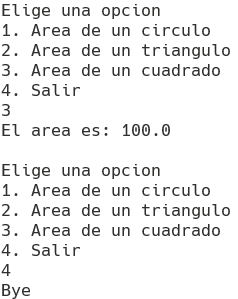
\includegraphics[width=0.4\columnwidth, center]{FG1.png}
  \end{figure}

  \subsection*{Ejercicio Práctico en el Lab}
  Calcular áreas de figuras geométricas usando la estructura de control \textit{switch} y entradas del usuario.

  \textbf{Código}
  \begin{lstlisting}
import java.util.Scanner;

public class FigurasGeometricas2 {
  static float area = 20;
  
  public static void main(String[] args) {
    float area = 0;
    int opcion;
    final float PI = 3.1415f;

    Scanner sc = new Scanner(System.in);
    do {
      System.out.println("Elige una opcion");
      System.out.println("1. Area de un circulo");
      System.out.println("2. Area de un triangulo");
      System.out.println("3. Area de un cuadrado");
      System.out.println("4. Salir");
      opcion = sc.nextInt();

      switch (opcion) {
        case 1:
          // Circulo
          float radio = 0;
          System.out.print("Ingrese el valor del radio: ");
          radio = sc.nextFloat();
          area = PI * radio * radio;
          break;
        case 2:
          // Triangulo
          float base = 0, altura = 0;
          System.out.print("Ingrese el valor de la base: ");
          base = sc.nextFloat();
          System.out.print("Ingrese el valor de la altura: ");
          altura = sc.nextFloat();
          area = (base * altura) / 2;
          break;
        case 3: 
          // Cuadrado
          float lado = 0;
          System.out.print("Ingrese el valor del lado: ");
          lado = sc.nextFloat();
          area = lado * lado;
          break;
        case 4:
          System.out.println("Bye");
          continue;
        default: 
          System.out.println("Su eleccion no existe");
          continue;
        }

      System.out.println("El area es: " + area + "\n");

    } while(opcion != 4);
    
    sc.close();
  }
} 
  \end{lstlisting}

  \textbf{Terminal}
  \begin{figure}[ht]
    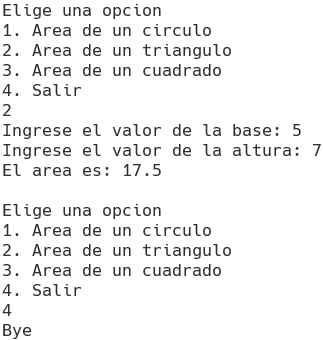
\includegraphics[width=0.5\columnwidth, center]{FG2.png}
  \end{figure} 

  Imprimir en la terminal los números primos en el rango que ingrese el usuario.

  \begin{lstlisting}
import java.util.Scanner;

public class Primos {
  public static void main(String[] args) {
    Scanner sc = new Scanner(System.in);

    int n;

    System.out.print("Ingrese el valor de n: ");
    n = sc.nextInt();

    for(int i = 2; i <= n; i ++) {
      if (i == 2 || i == 3 || i == 5 || i == 7) {
        System.out.print(i + " ");
        continue;
      }
      if (i % 2 == 0 || i % 3 == 0 || i % 5 == 0 || i % 7 == 0)
        continue;
      System.out.print(i + " ");
    }
    System.out.println();
    sc.close();
  }
}
  \end{lstlisting}

  \textbf{Terminal}
  \begin{figure}[ht]
    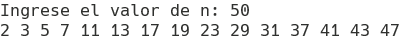
\includegraphics[width=0.75\columnwidth, center]{Primos.png}
  \end{figure} 

  \section*{Resultados}
  \subsection*{Problema 1}
  Elabore un programa que simule la compra de una tienda en línea. Considere al menos $20$ productos con sus costos. El cliente puede escoger n productos, al final deberá mostrarle cuanto es el total de su compra. Si la compra es mayor a $2,000$ pesos que se aplique un descuento del $5\%$ de la compra total, si la compra es mayor a $4,000$ pesos o más aplique un descuento del $7\%$. \textbf{Use la estructura de control \textit{Switch}}.

  \textbf{Explicación} \\


  \textbf{Código}
  % \begin{lstlisting}

  % \end{lstlisting}

  \textbf{Terminal}
  % \begin{figure}[ht]
  %   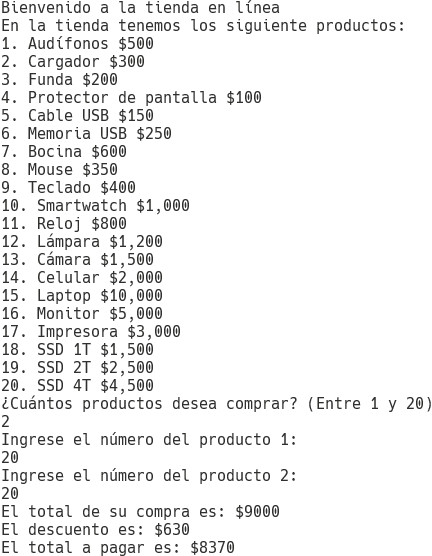
\includegraphics[width=0.75\columnwidth, center]{P1.png}
  % \end{figure}


  \subsection*{Problema 2}
  Elabore un programa que muestra la secuencia de la canción de navidad ``Twelve Days'', la canción tiene una estructura de rimas acumulativas, el narrador enumera los regalos que su amor ``verdadero'' le va enviando durante los doce días consecutivos de Navidad (entre las festividades de Navidad y la epifanía).

  Tome como referencia la siguiente foto:
  \begin{figure}[ht]
    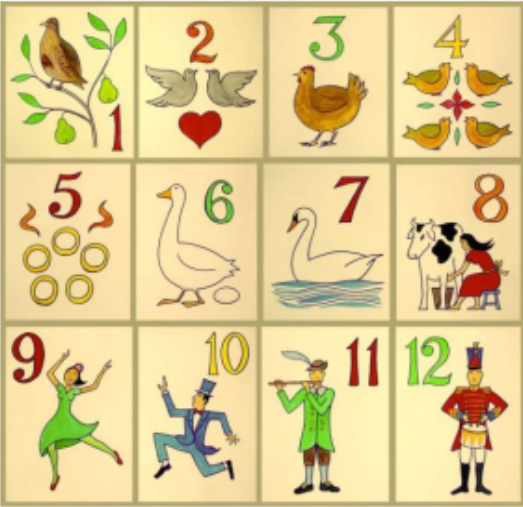
\includegraphics[width=0.6\columnwidth, center]{Cancion.png}
  \end{figure}

  \begin{enumerate}[label=\alph*)]
    \item Realice un primer programa que muestre en orden la secuencia de la canción de manera recursiva, donde cada estrofa añade un regalo y enumera todos los recibidos en las estrofas precedentes.
    \item Otro programa que realice orden aleatorio, es decir el día uno puede salir tres gallinas, el día dos puede salir diez señores saltando, sin olvidar repetir los regalos anteriores.
  \end{enumerate}

  \textbf{Use métodos de tipo \textit{static} y considere el uso de variables tipo \textit{final} para dichas implementaciones}.

  \subsection*{Versión A}

  \textbf{Explicación} \\
  Para mostrar cada estrofa se creo un método de tipo \textit{static} recursivo que se controla con un ciclo \textit{for} desde la el método \textit{main}. Los parámetros del método recursivo son el numero de la ultima estrofa y una variable iterativa que comienza desde $0$ y aumenta hasta ser igual al número de la ultima estrofa. Esto permite repetir las estrofas anteriores mientras se agregan las estrofas nuevas. 

  \textbf{Código}
  \begin{lstlisting}
public class Problema2VersionA {
  static void estrofas(int i, int j) {
    String estrofa = "";
    
    if(j >= i) {
      System.out.println();
      return;
    }

    switch(j) {
      case 0: estrofa = "Una perdiz en un peral"; break;
      case 1: estrofa = "Dos t\u00F3rtolas"; break;
      case 2: estrofa = "Tres gallinas francesas"; break;
      case 3: estrofa = "Cuatro p\u00E1jaros piando"; break;
      case 4: estrofa = "Cinco anillos de oro"; break;
      case 5: estrofa = "Seis ocas empollando"; break;
      case 6: estrofa = "Siete cisnes nadando"; break;
      case 7: estrofa = "Ocho sirvientas orde\u00F1ando"; break;
      case 8: estrofa = "Nueve damas danzando"; break;
      case 9: estrofa = "Diez se\u00F1ores saltando"; break;
      case 10: estrofa = "Once gaiteros tocando la gaita"; break;
      case 11: estrofa = "Doce tamborileros tocando el tambor";break;
    }
  
    System.out.println(estrofa);
    estrofas(i, j + 1);    
  }

  public static void main(String[] args) {
    for(int i = 1; i <= 12; i ++)
      estrofas(i, 0);
  }
}  
  \end{lstlisting}
  
  \textbf{Terminal}
  \begin{figure}[ht]
    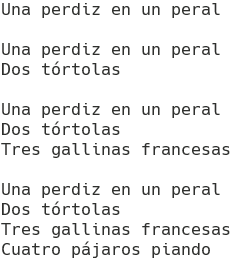
\includegraphics[width=0.38\columnwidth, center]{P2A.png}
  \end{figure}

  \subsection*{Versión B} 
  
  \textbf{Explicación} \\
  Para generar el orden aleatorio de las estrofas se crean 12 variables de tipo entero y se asignan con valores entre 1 y 12 sin repetirse, esto se hace mediante un ciclo \textit{while} que solo se termina cuando todas las variables son asignadas. El método para imprimir las estrofas es parecido a la versión A pero sin ser recursivo pues se controla por 2 ciclos \textit{for} y una estructura \textit{switch} en el método \textit{main}, lo que permite repetir las estrofas anteriores y llegar hasta las 12 estrofas.
  
  \textbf{Código}
  \begin{lstlisting}
import java.util.Random;

public class Problema2VersionB {
  static int n0, n1, n2, n3, n4, n5, n6, n7, n8, n9, n10, n11 = -1;

  static void estrofas(int i) {
    String estrofa = "";

    switch(i) {
      case 0: estrofa = "Una perdiz en un peral"; break;
      case 1: estrofa = "Dos t\u00F3rtolas"; break;
      case 2: estrofa = "Tres gallinas francesas"; break;
      case 3: estrofa = "Cuatro p\u00E1jaros piando"; break;
      case 4: estrofa = "Cinco anillos de oro"; break;
      case 5: estrofa = "Seis ocas empollando"; break;
      case 6: estrofa = "Siete cisnes nadando"; break;
      case 7: estrofa = "Ocho sirvientas orde\u00F1ando"; break;
      case 8: estrofa = "Nueve damas danzando"; break;
      case 9: estrofa = "Diez se\u00F1ores saltando"; break;
      case 10: estrofa = "Once gaiteros tocando la gaita"; break;
      case 11: estrofa = "Doce tamborileros tocando el tambor"; break;
    }
    
    System.out.println(estrofa); 
  }

  static void generarOrdenAleatorio() {
    Random rand = new Random();
    int i = 0;

    while (i < 12) {
      int n = rand.nextInt(12);
      boolean flag = true;

      if (n0 == n) flag = false;
      else if (n1 == n) flag = false;
      else if (n2 == n) flag = false;
      else if (n3 == n) flag = false;
      else if (n4 == n) flag = false;
      else if (n5 == n) flag = false;
      else if (n6 == n) flag = false;
      else if (n7 == n) flag = false;
      else if (n8 == n) flag = false;
      else if (n9 == n) flag = false;
      else if (n10 == n) flag = false;
      else if (n11 == n) flag = false;
      
      if (flag) {
        switch(i) {
          case 0: n0 = n; break;
          case 1: n1 = n; break;
          case 2: n2 = n; break;
          case 3: n3 = n; break;
          case 4: n4 = n; break;
          case 5: n5 = n; break;
          case 6: n6 = n; break;
          case 7: n7 = n; break;
          case 8: n8 = n; break;
          case 9: n9 = n; break;
          case 10: n10 = n; break;
          case 11: n11 = n; break;    
        }
        i ++;
      }
    }
  }
  
  public static void main(String[] args) {
    generarOrdenAleatorio();

    for(int i = 1; i <= 12; i ++) {
      for(int j = 0; j < i; j ++) {
        switch(j) {
          case 0: estrofas(n0); break;
          case 1: estrofas(n1); break;
          case 2: estrofas(n2); break;
          case 3: estrofas(n3); break;
          case 4: estrofas(n4); break;
          case 5: estrofas(n5); break;
          case 6: estrofas(n6); break;
          case 7: estrofas(n7); break;
          case 8: estrofas(n8); break;
          case 9: estrofas(n9); break;
          case 10: estrofas(n10); break;
          case 11: estrofas(n11); break;
        }
      }
      System.out.println();
    }
  }
}   
  \end{lstlisting}
  
  \textbf{Terminal}
  \begin{figure}[ht]
    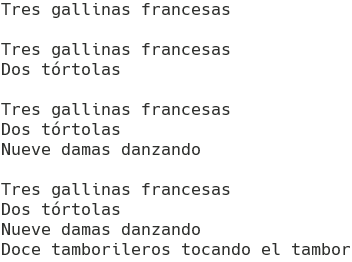
\includegraphics[width=0.55\columnwidth, center]{P2B.png}
  \end{figure}

  \subsection*{Problema 3}
  Realice el programa:  \href{https://edabit.com/challenge/48EJWLhF224na8po3}{Which Generation Are You?}. \textbf{Use operadores ternarios anidados}.

  \textbf{Explicación} \\
  Para resolver este problema se necesitan dos entradas de datos del usuario, el primero es un entero obligatoriamente entre $-3$ y $3$ y un carácter ``m'' o ``f''. Estos datos se pasan como parámetros a un método de tipo \textit{static} que primero accede a una estructura \textit{switch} para seleccionar la generación y luego por medio de un operador ternario se determina el sexo. Esta función retorna un \textit{String} que finalmente se imprime en el método \textit{main}.

  \textbf{Código}
  \begin{lstlisting}
import java.util.Scanner;

public class Problema3 {
  static String Generation(int n, char s) {
    switch(n) {
      case -3:
        return (s == 'm') ? "great grandfather" : "great grandmother";
      case -2:
        return (s == 'm') ? "grandfather" : "grandmother";
      case -1:
        return (s == 'm') ? "father" : "mother";
      case 0:
        return "me!";
      case 1:
        return (s == 'm') ? "son" : "daughter";
      case 2:
        return (s == 'm') ? "grandson" : "granddaughter";
      case 3:
        return (s == 'm') ? "great grandson" : "great granddaughter";
      default:
        return "";
    }
  }   

  public static void main(String[] args) {
    Scanner sc = new Scanner(System.in);
    int n;
    char s;
    
    do {
      System.out.print("Ingrese el numero de generacion (entre -3 y 3): ");
      n = sc.nextInt();

      if(n < -3 || n > 3)
        System.out.println("Error. Valor fuera de rango\n");
    } while (n < -3 || n > 3);

    do {
      System.out.print("Ingrese el sexo (m/f): ");
      s = sc.next().charAt(0);

      if(s != 'm' && s != 'f')
        System.out.println("Error. Valor invalido\n");
    } while (s != 'm' && s != 'f');

    System.out.println("\n" + Generation(n, s));
    sc.close();
  }
}    
  \end{lstlisting}

  \textbf{Terminal}
  \begin{figure}[ht]
    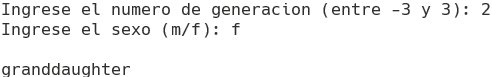
\includegraphics[width=0.8\columnwidth, center]{P3.png}
  \end{figure}

  \subsection*{Problema 4}
  Realice el programa:  \href{https://edabit.com/challenge/7CWbYfRji9yhna9tf}{Remove Trailing and Leading Zeros}. \textbf{Use operaciones \textit{casting}}.

  \textbf{Explicación} 
  

  \textbf{Código}
  % \begin{lstlisting}

  % \end{lstlisting}

  \textbf{Terminal}
  % \begin{figure}[ht]
  %   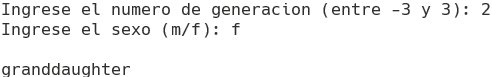
\includegraphics[width=0.75\columnwidth, center]{P3.png}
  % \end{figure}

  \subsection*{Problema 5}
  Realice el programa:  \href{https://edabit.com/challenge/48EJWLhF224na8po3}{Get the Date}. \textbf{Puede usar cualquier librería del API de JAVA}.

  \textbf{Explicación} \\
  Este código brinda la capacidad al usuario de ingresar una fecha siguiendo el formato ``DD/MM/YYYY''. A continuación, hace uso de la clase LocalDate y del objeto \textit{DateTimeFormatter} para llevar a cabo el análisis y la formateación de la fecha proporcionada. Una vez que se ha obtenido la fecha, se identifica el día de la semana correspondiente haciendo uso del método \textit{getDayOfWeek()}, el cual devuelve el nombre en inglés (por ejemplo, ``MONDAY'' para lunes). Posteriormente, se realiza una traducción de los nombres de los días de la semana al idioma español empleando una estructura \textit{if-else if}, lo que conlleva la conversión de ``MONDAY'' a ``Lunes'', ``TUESDAY'' a ``Martes'', y de manera sucesiva. Por último, se presenta en la pantalla el día de la semana en español. 
  

  \textbf{Código}
  \begin{lstlisting}
import java.time.LocalDate;
import java.time.format.DateTimeFormatter;
import java.util.Scanner;

public class Problema5 {

  public static void main(String[] args) {
    Scanner scanner = new Scanner(System.in);

    System.out.print("Ingresa la fecha (DD/MM/YYYY): ");
    String fechaInput = scanner.nextLine();

    DateTimeFormatter dateFormat = DateTimeFormatter.ofPattern("dd/MM/yyyy");

    LocalDate fecha = LocalDate.parse(fechaInput, dateFormat);
    String diaDeLaSemana = fecha.getDayOfWeek().toString();
    
    if (diaDeLaSemana.equals("MONDAY")) {
      diaDeLaSemana = "Lunes";
    } else if (diaDeLaSemana.equals("TUESDAY")) {
      diaDeLaSemana = "Martes";
    } else if (diaDeLaSemana.equals("WEDNESDAY")) {
      diaDeLaSemana = "Miercoles";
    } else if (diaDeLaSemana.equals("THURSDAY")) {
      diaDeLaSemana = "Jueves";
    } else if (diaDeLaSemana.equals("FRIDAY")) {
      diaDeLaSemana = "Viernes";
    } else if (diaDeLaSemana.equals("SATURDAY")) {
      diaDeLaSemana = "Sabado";
    } else if (diaDeLaSemana.equals("SUNDAY")) {
      diaDeLaSemana = "Domingo";
    }
    
    System.out.println("El dia de la semana es: " + diaDeLaSemana);
    scanner.close();
  }
}
  \end{lstlisting}

  \textbf{Terminal}
  \begin{figure}[ht]
    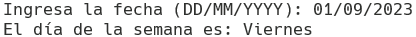
\includegraphics[width=0.75\columnwidth, center]{P5.png}
  \end{figure}


  \section*{Conclusiones}
  La elaboración de programas en el lenguaje Java que incorporen variables y constantes de diversos tipos de datos, expresiones y estructuras de control de flujo se erige como un pilar fundamental para cualquier desarrollador que trabaje con esta tecnología. Este objetivo esencial constituye los fundamentos de la programación en Java, otorgando las herramientas esenciales para la concepción de aplicaciones sólidas y operativas.

  La comprensión de la variedad de tipos de datos disponibles y su aplicación apropiada habilita a los programadores para gestionar un amplio espectro de información, que abarca desde números y cadenas de texto hasta estructuras de datos más complejas. Del mismo modo, la capacidad para crear expresiones y emplear operadores facilita la manipulación y transformación eficaz de los datos.

  En cuanto a las estructuras de control de flujo, como las sentencias condicionales y los bucles, desempeñan un papel crítico en la regulación de la secuencia de ejecución de un programa. Estas construcciones posibilitan que las aplicaciones tomen decisiones y repitan tareas de forma eficiente, lo que resulta esencial para la creación de software interactivo y dinámico.

  \section*{Referencias}
  \small
  Jeroen Ndh. \textit{Which Generation Are You?}. Edabit. \url{https://edabit.com/challenge/48EJWLhF224na8po3} \\

  Mubashir Hassan. \textit{Mubashir's Mystery Challenge}. Edabit. \url{https://edabit.com/challenge/7CWbYfRji9yhna9tf} \\

  DreamArdor. \textit{Get the Date}. Edabit. \url{https://edabit.com/challenge/K8FPxyGNDXhWQD9jX}
\end{document}